\subsection{\Dc}
\begin{figure}[tb]
	\centering
	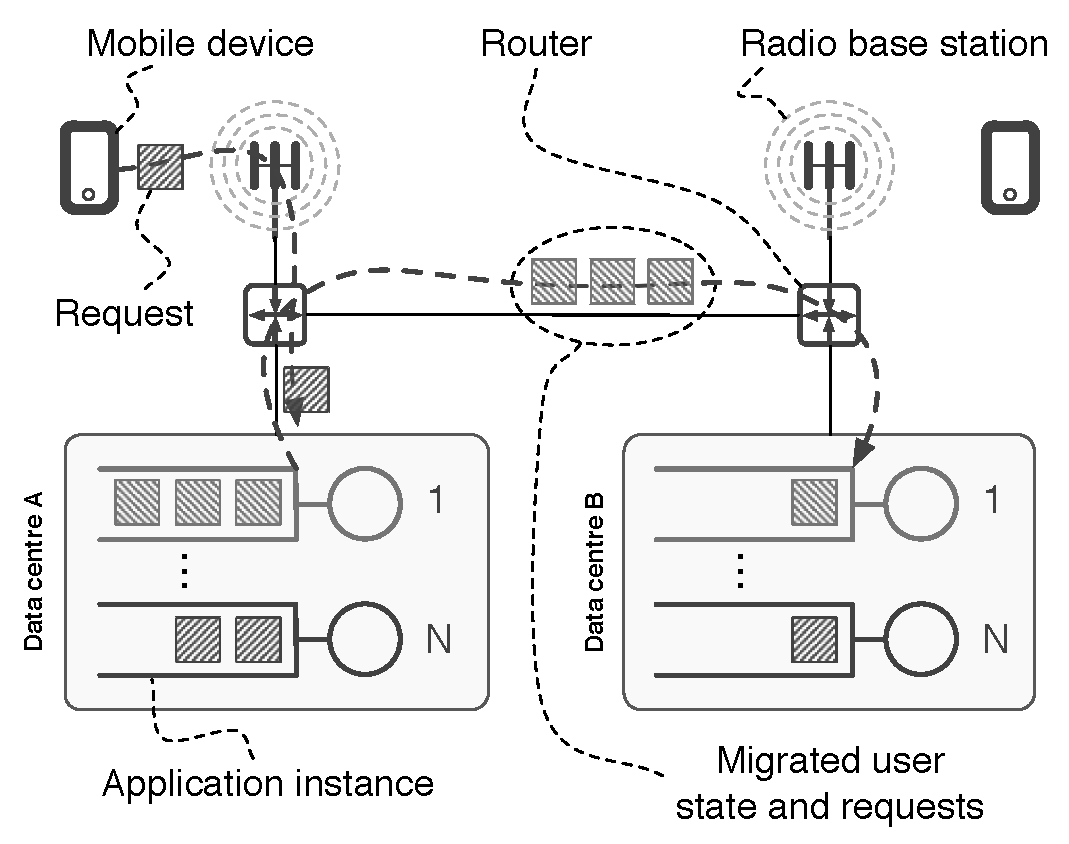
\includegraphics[width=\linewidth]{fig_dc_model.eps} 
	\caption{\Dc{} model}
	\label{fig:dc_model}
\end{figure}

We model a \dc{} using two parameters, the number of CPUs and their speed (in FLOPS or MIPS).
We assume that all CPUs in one \dc{} are identical, we do not represent that they are located in separate physical machines (servers) and we do not consider memory, storage and intra \dc{} network.

%As illustrated in Figure \ref{fig:dc_model}, a \dc{} is modelled as a series of parallel queues, one for each allotted VM, and thus, service $N_{i,vm}$. 
%A dispatcher directs incoming requests to the corresponding VM based on which service $S_j$ it carries. 
%In normal operation, each request is served by its associated queue with a service time of $T_{i,vm}$, unique to the $i_{th}$ \dc{} and is proportional to the number of VMs $N_{i,vm}$ running concurrently in the \dc{} in excess of $N_{ser}$.
%When the queue in a VM or subset of VMs in a \dc{} $N_{i,sus vm} \subset N_{i,vm}$ are temprarily empty, the remaining VMs will be rewarded with a reduction in service time propotinal the number of suspended VMs $T_{sus} \propto N_{i,sus vm}$.

%To simplify the model of a \dc{} we do not consider CPU, memory, storage and intra \dc{} network separately.
%Instead, in this paper, we will use an abstraction of one dimensional computational resource.

\subsubsection{Hosting applications in a \dc{}}
%Hosting VMs in a \dc{} can be modeled in two ways: with or without competition for computational resource.

%In the first approach, the resources of a \dc{} are aggregated in one pool that is continuously divisible.
%Each VM gets an equal part of available resources inversely proportional to the number of VMs hosted in the data center.
%The bigger is the number of VMs hosted in the \dc{}, the smaller amount of resources each of them gets.
%The pool of resources is divided evenly among all VMs.
%Hence, when the number of VMs hosted in the \dc{} increases, the amount of resources available for each VM shrinks.
%Consequently the service time of processing requests of each VM lengthens.

%In the second approach, the resources of a \dc{} are discrete and each computational unit is used exclusively by one VM.
%Therefore, there is no influence of one VM on another.
%To incorporate the fact that the amount of resources is finite we put a limit on the maximal number of VMs that can be hosted in one \dc{}.
%Furthermore, on each \dc each service is contained within one VM. 
Applications are hosted on the resources located in the \dcs{}.
The time that is necessary for serving an application request depends on the CPU speed of a hosting machine.
The capacity of a \dc{} is determined by the number of available CPUs. 
%New instances of application are not accepted when the capacity of a \dc{} is reached.
%Limitation of the number of hosted application instances
%Strong limit --- The capacity of \dc{} is determined by the number of available CPUs. New instances of application are not accepted when the capacity of DC is reached.
%Flexible limit --- When the nominal capacity of DC is reached accepting new applications causes increase of the service time for all hosted application instances.

%\begin{equation}
%T_{serv} = \frac{max \lbrace \#CPUs, \#APPs \rbrace}{\#APPs} \cdot basic\_service\_time
%\end{equation}

Computation resources of a \dc{} are virtualized and each application instance runs inside of its own Virtual Machine (VM). Each VM is mapped to one physical CPU, so the maximal number of VMs, that can be hosted in a \dc{}, is equal to the number of CPUs.

%\subsubsection{Overhead of VM start, stop, and migration}
%\subsubsection{Overhead of VM initialization and migration}
\subsubsection{VM initialization and termination}
%When a request from a previously unknown service $S_j$ is served to a \dc{}, a new VM will be started to host that service.
In our scenario a VM hosts a service that can be concurrently accessed by many users.
A VM is initialized upon receiving the first request from a client and terminated when there are no more requests to serve (waiting queue is empty and all sessions are finished).

When a decision of deploying a new service in a \dc{} is taken, a new VM will be started there to host an application instance of that service.
Due to the startup time, the newly admitted VM will not be able to start processing requests for a period of $T_{vm\_init}$. 
%Nevertheless, the base VM service time for the \dc{} $T_{i,vm}$, will be adjusted to the for the new VM count.
Nevertheless, the new VM will start using resources of the \dc{} from the time of admission.
%Because of that, the service time, $T_{i,vm}$, for each of the VMs hosted in that \dc{} will be recalculated to reflect the temporary load scenario.
Similarly, after finishing serving the last request, the VM will still be using the resources of the \dc{} for time $T_{vm\_release}$.

%\subsubsection{VM activation scheme}
%Definitions: service, session, client subscribed to service 

%%\begin{enumerate}
%%	\item Private VM
%\textbf{Private VM} --- IaaS like, a VM is exclusively used by one user for offloading computations from his \ue{}.
%User provides the executable program that is loaded to an edge \dc{} from an \ue{} or a remote \dc{}.
%		\begin{description}
%			\item \textbf{per-session} --- a VM is initialized upon receiving the first request from a client and terminated just after finishing processing the last request of the session.
%			\item \textbf{client-within-cell} --- a VM is initialized when a client that is subscribed to a service enters a cell and is kept alive as long as he stays within the cell. 
%		\end{description}
%			
%%	\item Shared VM
%\textbf{Shared VM} --- SaaS like, a VM hosts a service that can be concurrently accessed by many users.
%		\begin{description}
%			\item \textbf{any-client-running} --- a VM is initialized upon receiving the first request from a client and terminated when there are no more requests to serve (waiting queue is empty and all sessions are finished).
%			\item \textbf{any-client-within-cell} --- a VM is initialized when the first client that is subscribed to a service enters a cell and is kept alive as long as any subscribed client stays within the cell. 
%		\end{description}
%%\end{enumerate}

\subsubsection{Requests and user state migration}

%\subsubsection{VM migration}
%Migration has an influence on the service performance as well as on the resource availability on both source and destination \dc{}.
%On the source side, apart from ordinary resource requirements due to serving requests, VM consumes resources for sending its image to the destination \dc{}.
%In a case of postcopy live migration, VM at the source side still uses some resources even after the workload is redirected to the new location.
%That is because the VM at the destination side pulls remaining memory pages from the source \dc{}.

%The overhead of VM migration can be modeled in different ways depending on the manner how \dc resources are represented.

%To model the overhead of migration on the service performance additional delay in the response time should be introduced.
%Primarily, during the phase of transferring the image of VM, because of using a part of resources for I/O operations.
%Primarily, for the time of transferring the image of VM, $T_{vm\_transfer}$, the time of serving a request should be lengthen by $D_{vm\_transfer}$, because of using a part of resources for I/O operations.
%Moreover, during the time of switching the execution from the source to the destination, $T_{vm\_downtime}$, VM is not able to serve any requests.
%Additionally, in the case of the postcopy migration, delay occurs also for some time after redirecting the workload to the new \dc{}, due to the remote memory calls.
%Additionally, in the case of the postcopy migration, delay  $D_{memory\_pull}$ occurs for some number, $N_{memory\_pull}$, of the first requests after redirecting the workload to the new \dc{}, due to the remote memory calls.

%That can be modeled by running two instances of VM during the time of migration, one per each DC.
%When VMs compete for resources, running additional VM on the destination side introduces an overhead by increasing the response time of other collocated VMs.

The statefulness of the service dictates the amount of information that needs to be migrated to the succeeding \dc{}.
The $H$ parameter in Equation \ref{eq:vm_util_comp}, is the state entropy of the communication between a \ue{} and a \dc{} which thus dictates the scale of the incurred overhead when migrating that users state the receiving \dc{}.